\documentclass[10pt,aspectratio=169]{beamer}

% All the boilerplate is in ccaslides.sty
% Note that this also pulls in a custom vogtwidebar.sty
\usepackage{ccaslides}

\author{Ji\v{r}\'i Lebl}

\institute[OSU]{%
Departemento pri Matematiko de Oklahoma {\^S}tata Universitato}

\title{Cultivating Complex Analysis:\\%
The argument (1.2.3)\\%
Mapping properties of the exponential (1.2.4)}

\date{}

\begin{document}

\begin{frame}
\titlepage
\end{frame}

\begin{frame}
We attempt to define the argument of $z = re^{i\theta}$:
\begin{equation*}
\arg z
\overset{\text{def?}}{=}
\theta ,
\end{equation*}
\pause
But if $\theta$ is an argument of $z$,
then so is $\theta+2\pi$, $\theta-2\pi$, or $\theta + k 2\pi$ for any $k \in
\Z$.

\medskip
\pause

$\arg z$ is not a function but a \emph{multivalued function}:
\begin{equation*}
\arg z
\overset{\text{def}}{=}
\ldots,\theta - 4\pi,
\theta - 2\pi,
\theta ,
\theta + 2\pi,
\theta + 4\pi, \ldots
\end{equation*}

\pause

Note that $\arg 0$ is undefined.

\end{frame}

\begin{frame}
To try to solve the multivaluedness, we define the
\emph{principal branch of $\arg$}:
\begin{equation*}
\Arg z
\overset{\text{def}}{=}
\theta, \qquad \text{where } -\pi < \theta \leq \pi.
\end{equation*}

\pause

A good attempt.

\medskip

Alas $\Arg$ is discontinuous

on the negative real axis.


\vspace*{-0.5in}
\hspace*{2.7in}%
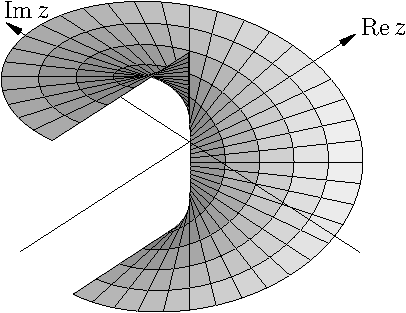
\includegraphics[width=2.5in]{../figures/arggraph}

\pause

\vspace*{-0.8in}

\textbf{Remark:} Some authors make principal

branch take values in $[0,2\pi)$.

\end{frame}

\begin{frame}
Let's see what the exponential does to $\C$.

\medskip
\pause

$e^{z+w} = e^z e^w$ implies $e^z$ is never zero (exercise).

\medskip
\pause

In fact, the complex exponential is onto $\C \setminus \{ 0 \}$.

\medskip
\pause

The complex exponential is not one-to-one, it is 
infinitely-many-to-one.  For any integer $k$,
\[
e^{z+ik2\pi} = 
e^{z} e^{ik2\pi} =
e^z .
\]

\end{frame}

\begin{frame}
$
e^{z} = 
e^{x+iy} =
e^x e^{iy}  %\qquad \text{and} \qquad \sabs{e^{iy}} =1 
$

\medskip
\pause
So $e^z$ takes a vertical line, $x=c$, to 

the circle of radius $e^c$.

\vspace*{-0.5in}
\hspace*{2.35in}
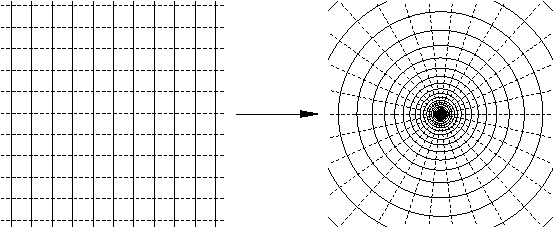
\includegraphics[width=3.3in]{../figures/expplotlines}

\vspace*{-0.8in}


\pause

It takes the strip $a < x < b$ to the

annulus
$
\bigl\{ w \in \C : e^a < \sabs{w} < e^b \bigr\} .
$

\medskip
\pause

It takes a horizontal line, $y=c$, to

a ray from the origin, $\theta=c$.

\pause
\medskip

So the strip $a < y < b$ goes to the sector
$
\bigl\{ w \in \C : ``a < \arg w < b'' \bigr\} .
$

\medskip
\pause

\textbf{Remark:}
$e^z$ takes the set given by
$2k\pi < \Im z \leq 2(k+1)\pi$ in a one-to-one way onto
$\C \setminus \{ 0 \}$.


\end{frame}

\end{document}
